\chapter{Analysis}
This chapter provides the background knowledge required to understand the thought process behind the selected technologies.
The group have been advising the assignment provider as to suitable technologies for the project but the assignment provider has been the one selecting them.
The chapter first inspects the database technologies that are suitable for the assignment.
Afterwards the chapter examines the selected frontend technology before analyzing the technology stack used for the backend development.
Lastly the chapter provides insight as to why the methodology selected is the most suitable for the project.

\section{Database technology selection}
The two most popular database systems today are the SQL- and NoSQL-based database systems \cite{stackoverflow-db-statistics}.
The distinction between SQL and NoSQL database systems have become increasingly blurred \cite{sql-vs-nosql}, but there are still key differences between the two which makes them worth analyzing in order to find the most suitable database system for this project.

\iffalse
\subsection{CAP theorem}
The CAP theorem is a theorem within distributed database systems \cite{sql-schema}.
The theorem states that only two out of the following conditions can hold at any time:
\begin{itemize}
    \item Availability.
    This condition states that every request receives a (non-error) response.
    This means the data requested may not necessarily be up-to-date as the node may not have the up-to-date data \cite{sql-schema}.
    \item Consistency.
    This condition states that all nodes have access to the same data.
    This means whenever an attempt to extract data from the database is made the database will either provide up-to-date data or failure \cite{sql-schema}.
    \item Partitioning tolerance.
    This condition states that the database system will continue to operate despite any number of messages between the nodes being delayed or dropped by the network.
    This means the database system can operate normally while sustaining any number of network failures so long as not every node is experiencing failure \cite{sql-schema}.
\end{itemize}

A database is said to support AC when availability and consistency are selected, its said to support AP when availability and partitioning tolerance are selected and its said to support CP when consistency and partitioning tolerance are selected.
\fi

\subsection{SQL} 
SQL(Structured Query Language) is a database language for data management\cite{sql-goal} of a RDBMS(relational database management system) \cite{sql-is-a-rdbms} based on the relational data model proposed by Edgar Frank Todd \cite{rdbms}.
The relational data model logically structures all relations(tables) and each relation is provided a name and is built up of named attributes - columns of data \cite{sql-is-a-rdbms}.
The rows of a table are known as tuples \cite{sql-is-a-rdbms} and, provided the table is normalized for the first normal form or higher, they contain one value per attribute \cite{sql-1nf}.
The figure attached below illustrates the relational model further.

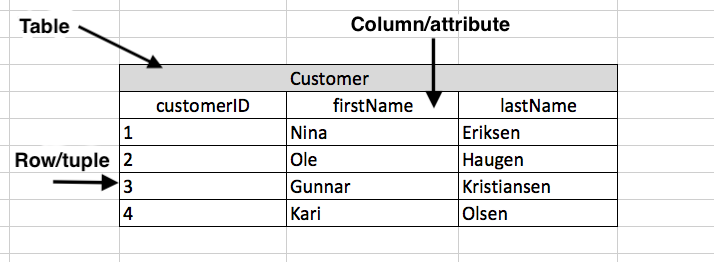
\includegraphics[width=115mm,scale=1]{figures/relational-db-visualised.png}

\textit{Figure nr. (TODO): Displays a table named "Customer", with three attributes and four tuples.}

SQL offers a data definition language(DDL) \cite{sql-components}.
The DDL defines the database schema - that is the structure, meaning which attributes the tables consists of, and which tables the database consists of.
It is impossible to add data to the database until a schema has been defined.
The DDL also describes any relational integrities the tables of the database, or the columns of table, may have \cite{sql-constraints}.
In the figure below a given customer may have several orders but a given order may have one and only one customer associated with it; this is an example of a one-to-many relationship.
In addition to a one-to-many relationship an attribute or table may also have a one-to-one or a many-to-many relationship \cite{sql-relationships}.
Lastly the DDL also defines any security constraints the database may have - such as which users have permissions to read, update or delete the contents of a given table \cite{sql-ddl}.

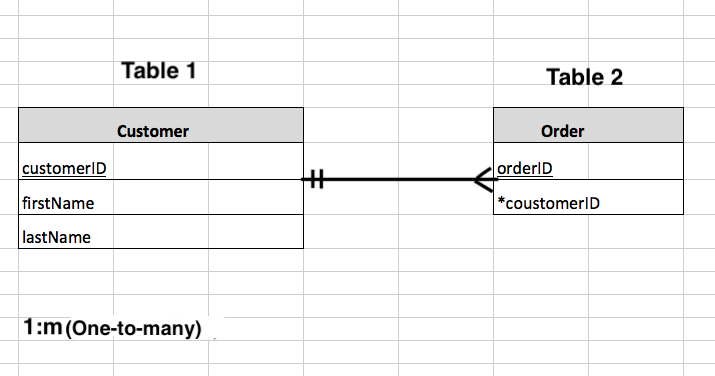
\includegraphics[width=115mm,scale=1]{figures/relational-db-relation.png}

\textit{Figure nr. (TODO): Displays a one-to-many relation between customer and orders}

SQL also offers a data manipulation language(DML) \cite{sql-components}.
The DML allows for the insertion of, retrieval of, update of, and deletion of data \cite{sql-dml-options}.
Whenever a tuple is added, updated or removed the tuple must conform to the restraints set by the DDL.
The attempted action will be aborted should there be discrepancies between the constraint of the table or column and the data.
This ensures that the data in the table is accurate and reliable \cite{sql-constraints}.

In addition SQL:
\begin{itemize}
    \item Provides an organized structure as data is defined once, and items referencing the data does so using foreign keys \cite{upwork-sql-adv}.
    \item Reduces data redundancy due to the organized structure \cite{upwork-sql-adv}.
    \item Allows JOIN operations \cite{upwork-sql-adv}.
    The operation allows two or more tables to be combined based on some shared attribute between them.
    The JOIN operation provides the ability to fetch specific data across tables that otherwise would prove cumbersome \cite{sql-joins}.
    \item Provides support for transactions.
    Transactions are essential in databases which require reliable data as they provide a framework for an all-or-nothing approach.
    This means the sequence of involved operations have to succeed in its entirety.
    The database will perform a rollback and raise an error should one of the operations fail \cite{sql-transactions}.
\end{itemize}

\subsection{NoSQL}
A NoSQL(Not only SQL) database provides data storage and data retrieval capabilities that is not modeled using a conventional RDBMS \cite{nosql-not-rdbms}.
Schema-less models are used instead of the traditional RDBMSs.
The most popular models include:
\begin{itemize}
    \item Key-value stores.
    Every item in the database is stored as an attribute name with a corresponding value \cite{mongodb-explains-nosql}.
    The key and value can be anything, and the key acts as a unique identifier for the value \cite{nosql-key-value}.
    \item Document databases.
    Document databases are an extension to key-value stores.
    Documents are structures which can contain many different key-pairs, and documents can even contain other documents.
    The documents can store data in different format, such as XML or JSON.
    Document databases are intended to store semi-sorted data \cite{nosql-document-sort}.
    \item Wide-column stores.
    The data in the database is stored in columns rather than the typical SQL rows.
    A given row can therefore have columns that other rows does not have.
    A wide-column store can be considered a two-dimensional key-value store \cite{infoworld-sql-vs-nosql}.
    \item Graph stores.
    The data in the database is represented as a graph.
    Their intended use is to traverse and navigate relationships.
    These databases use nodes to represent items in the database, and an edge between two nodes represents a relationship between the two items \cite{nosql-graph}.
\end{itemize}

NoSQL is advantageous because it:
\begin{itemize}
    \item Allows for semi-structured or unstructured data in the database.
    This flexible design allows the database to handle changes in structure more easily, and also allows the database to scale with ease \cite{mongodb-adv-nosql}.
    \item Allows for data to be inserted without a schema \cite{omkarsoft-adv-nosql}.
    This is beneficial should data be expected to change during the development of the project.
    \item Scales horizontally rather than vertically \cite{mongodb-adv-nosql}.
    Scaling horizontally allows partitions of data to be scatted across several pieces of hardware in order to store the data in the database.
    By contrast, scaling vertically means replacing already-existing hardware with more powerful hardware \cite{technopedia-nosql-scale}.
    %\item Some operations in NoSQL is faster than SQL, because the data structures are different. \cite{Amazon DynamoDB}
    %\item NoSQL has the ability to perform ad-hoc joins across tables. \cite{Data management in cloud}
\end{itemize}

\subsection{Why SQL is the selected database system}
The group have looked into both SQL and the NoSQL to find out what fits the project best and also consulted with the assignment provider. Since the project is to create a lending system for the school, the group believe that for this system it won’t contain large amount of data. The data will contain information about the student, employees and the equipment that you can find in MakerSpace. In other words, there are not millions of data that will be stored, and the group don’t see the need for a NoSQL system. SQL is however a standardized database query system and because of this the adaptability of SQL is great\cite{structured-query-language}. If SQL lacks a feature there is nothing keeping it back from being improved upon. The support for SQL is not going to suddenly stop and is used in most known database management systems today. This ensures that support for SQL and DBMS is not going to halt the project or stop the product from functioning in the future.  

The group don’t believe that the lending will contain allot of tables and relation either, but also don’t see how NoSQL benefits more than a SQL system will. By choosing a SQL system instead of a NoSQL, it will avoid a lot of duplicates too, since NoSQL duplicate a lot of data.

\subsection{MariaDB as software}
After that the group found out that they wanted to use a SQL system for the project and as the assignment provider 
agree with, the group had to look away from MongoDB, since MongoDB is a NoSQL system, the group needed to find another solution. When researching into what software to use, the group found MariaDB as a good alternative. The assignement provider was consulted and agreed that MariaDb was a good choice. MariaDB is an open source software and also one of the most popular database servers you can find in this world. Since MariaDB has been made by the original developers of MySQL, MySQL and MariaDB shares the same structure. They use the same query and if you already have MySQL there is no problem switching to a MariaDB server. MariaDB can be seen as MySQL, just with some more functionality. Because of the plugins and tools MariaDB make it very open for a wide variety of uses. MariaDB also support javascript and node.js. This is important for the project since the group will use both. As a conclusion, the group don't see the need for MySQL when MariaDB covers all functionality that MySQL have, and also offers more than MySQL does. The choice of a Database ended with MariaDB.\cite{mariadb_1}\cite{mariadb_2}

\section{Choice of frontend} 
\todo{Legg til bilder på frontend og backend}
\todo{Event loop for backend og reactivity for frontend}
For the frontend technology the group had several choices, since the group earlier had decided to go for a full JavaScript technology stack and the assignment provider agreed with the choice. This did not limit our choice for a frontend technology since there are alot of frontend frameworks written in JavaScript. The group ended up debating between React and Vue.js. Both React and Vue.js are very similar but does things differently. 

 Vue.js was chosen because of three major factors; the size of the framework, live updating in the browser and the low learning curve in the start. Vue.js is comparably smaller than many of the other big JavaScript frameworks out there. It is roughly 58.8 kB in size. Since the framework is so small it will help with the loading speed of the web application. The second major point for choosing Vue.js was the reactivity of Vue. With the reactivity of Vue.js you could update individual components based off of which data had been updated in the database. With this feature there will be no need to update the whole site to show an update in the database. The last major point for the group was the low learning curve of Vue.js. With this learning curve it means that the easier parts of Vue.js is easier to learn, but the more complicated components can be harder. This is perfect for the groups project since all the group members are new to Vue.js and can faster get into the programming.

\section{Choice of backend}
For the backend technology there are several technologies that could be used. The group had discussed what back-end technology to use, and asked the assignment provider to choose. A full JavaScript technology stack was chosen and some of the major backend technologies have been ruled out. Such as Pythons Django, PHP or Javas Spring backend framework. 

JavaScript will be used for the backend, Node.js will be used as the server to create and handle the backend operations needed in the application. Node.js is a JavaScript run-time environment that can run JavaScript code outside of the browser using the V8 JavaScript engine. Node.js runs on a single thread and is able to do this because of the Event Loop. The event loop is how Node.js gets a request, it will make that request into a task and delegate it to another part of the system it runs on. When the task is done the feedback get sent back to Node.js and Node sends that back to the recipient. The reason this event loop is so efficient at handling requests is because it runs asynchronous. So when it receives a request and sends off a callback function for that request. It doesn't need to wait for that callback function to return something before it handles a new request.

\section{Analysis of different MakerSpaces}
The project group has decided to conduct interviews with different MakerSpace branches in Norway. The reason for choosing interviews is to be able to decide what information we want to get out of the interviewees. The project group will make a set of predetermined questions about how MakerSpace operates and what kind of systems and technologies they have. While conducting the interviews the project group also wants to arrange the interview at the respective MakerSpace, where the project group could get a tour of the MakerSpace and take a look at the systems they have and how they are used. This will be used to get more hands-on knowledge for the project, to be able to make a better system. The interviewee will also be more comfortable in a known environment during the interview. 

\subsection{Interview method}

\todo{Unngå små avsnitt}
Interviews can be defined as a qualitative research technique. This involves conducting intensive individual interviews with a small number of respondents to explore their perspectives on a particular idea, program or situation.\cite{Interview-Methods} Interviews have three different formats: structured, semi-structured and unstructured.

Unstructured interviews is conducted without any questions prepared before the interview takes place and data is collected in an informal way. This makes unstructured interviews very unreliable from a research standpoint. Answers given during an interview will also vary based on the formulation of the question. Comparing the answers for the questions will then be a challenge due to the different formulation.

Semi-structured interview is like a mix of structured and unstructured interviews. Questions are prepared before an interview and additional questions might be asked during the interview to either clarify, specify or expand on a certain question. 

Structured interviews consists of a set of predetermined questions that all of the interviewees will answer. The questions will be asked in the same order for every interviewee. The data collected from the answers will make data analysis easier because comparing the questions is straightforward. And it is easier to see the contrast between the different answers given.

Interviewing people for the project will have many advantages like the chance to collect detailed information about what other MakerSpaces do, and what kind of systems is in place for loaning out equipment or if they even have a system. By interviewing different MakerSpaces the group has more direct control over the flow of the interview process and has a chance to clarify issues during the interview process. This will make the data collected more accurate and easier to compare to the answers of other MakerSpace branches.

There is however some disadvantages of conducting interviews. One of the disadvantages is the time needed to arrange the interviews at appropriate times for the interviewees and the project group. Each member of the project group would learn most by being present in all the interviews. Being able to see and listen to what other MakerSpaces do would be a better experience than reading a summary or written answers to the interview. Depending on the time needed for other tasks for the project and the interview. The project group will send one person to all the interviews if time is limited.    
